\documentclass[11pt,letterpaper]{article}
\usepackage[utf8]{inputenc}
\usepackage[T1]{fontenc}
\usepackage[spanish]{babel}
\usepackage{amsmath}
\usepackage{amsfonts}
\usepackage{amssymb}
\usepackage{graphicx}
\usepackage{lmodern}
\usepackage{xspace}
\usepackage{multicol}
\usepackage{hyperref}
\usepackage{float}
\usepackage{hyperref}
\usepackage{color}
\usepackage{framed}
\usepackage[thinc]{esdiff}	
\DeclareUnicodeCharacter{2212}{-}

\usepackage{biblatex}
\addbibresource{bibliografia_proyecto_inferencia.bib}
\DeclareUnicodeCharacter{0301}{\'{i}}
\usepackage{enumerate}% http://ctan.org/pkg/enumerate

\usepackage[left=2cm,right=2cm,top=2cm,bottom=2cm]{geometry}

\newcommand{\X}{\mathbb{X}}
\newcommand{\x}{\mathbf{x}}
\newcommand{\Y}{\mathbf{Y}}
\newcommand{\y}{\mathbf{y}}
\newcommand{\xbarn}{\bar{x}_n}
\newcommand{\ybarn}{\bar{y}_n}
\newcommand{\paren}[1]{\left( #1 \right)}
\newcommand{\llaves}[1]{\left\lbrace #1 \right\rbrace}
\newcommand{\barra}{\,\vert\,}
\newcommand{\mP}{\mathbb{P}}
\newcommand{\mE}{\mathbb{E}}
\newcommand{\mR}{\mathbb{R}}
\newcommand{\mJ}{\mathbf{J}}
\newcommand{\mX}{\mathbf{X}}
\newcommand{\mS}{\mathbf{S}}
\newcommand{\mA}{\mathbf{A}}
\newcommand{\unos}{\boldsymbol{1}}
\newcommand{\xbarnv}{\bar{\mathbf{x}}_n}
\newcommand{\abs}[1]{\left\vert #1 \right\vert}
\newcommand{\muv}{\boldsymbol{\mu}}
\newcommand{\mcov}{\boldsymbol{\Sigma}}
\newcommand{\vbet}{\boldsymbol{\beta}}
\newcommand{\veps}{\boldsymbol{\epsilon}}
\newcommand{\mcC}{\mathcal{C}}
\newcommand{\mcR}{\mathcal{R}}
\newcommand{\mcN}{\mathcal{N}}

\newcommand{\ceros}{\boldsymbol{0}}
\newcommand{\mH}{\mathbf{H}}
\newcommand{\ve}{\mathbf{e}}
\newcommand{\avec}{\mathbf{a}}
\newcommand{\res}{\textbf{RESPUESTA}\\}

\newcommand{\defi}[3]{\textbf{Definición:#3}}
\newcommand{\fin}{$\blacksquare.$}
\newcommand{\finf}{\blacksquare.}
\newcommand{\tr}{\text{tr}}
\newcommand*{\temp}{\multicolumn{1}{r|}{}}
\newtheorem{ej}{Ejemplo}[section]
\newcommand{\grstep}[2][\relax]{%
   \ensuremath{\mathrel{
       {\mathop{\longrightarrow}\limits^{#2\mathstrut}_{
                                     \begin{subarray}{l} #1 \end{subarray}}}}}}
\newcommand{\swap}{\leftrightarrow}

\newcommand{\gen}{\text{gen}}
\newtheorem{thmt}{Teorema:}
\newtheorem{thmd}{Definición:}
\newtheorem{thml}{Lema:}
\newtheorem{thme}{Ejemplo:}
\title{Comparaciones Múltiples desde la perspectiva de Ciencia de Datos y su relación con el False Discovery Rate.}
\author{Edgar Steven Baquero Acevedo \and Enrique Santibáñez Cortés}

\begin{document}
\maketitle
\section{Introducción}
Parte del estudio de la inferencia estadística está relacionada con el cuestionamiento del espacio de parámetros que estimamos a través de los datos. Es así, como la formalización de una pregunta se vuelve conveniente desde el punto de vista teórico, pues nos permite abordar preguntas con el rigor necesario para tomar una decisión. Esta formalización puede ser llevada a cabo por procedimientos estadísticos con el fin de juzgar si una propiedad se satisface para una población, con base en lo observado por una muestra de dicha población.

El procedimiento anteriormente nombrado, es conocido como \textit{prueba de hipótesis}, y mediante esta teoría, es posible abordar problemas estadísticos, considerando una hipótesis nula y una alternativa, que luego definiremos con más detalle. Extendiendo un poco más este concepto, nos encontramos con la teoría de pruebas de hipótesis múltiples (PHM o MCP por sus siglas en inglés), de la cual, se ha desarrollado mucha investigación, sobretodo en los últimos años, donde ha presentado su auge en trabajos relacionados al de Benjamini y Hochberg (Ver \cite{BH}).%referencia artículo BH

El procedimiento se presenta cuando consideramos un conjunto de inferencias de manera simultánea (ver \cite{Miller} ) % Miller, R.G. (1981). Simultaneous Statistical Inference 2nd Ed. Springer Verlag New York. ISBN 978-0-387-90548-8.
 o se infiere un subconjunto de parámetros basados en valores observados (Ver por ejemplo \cite{Benjamini-2010});% Benjamini, Y. (2010). "Simultaneous and selective inference: Current successes and future challenges". Biometrical Journal. 52 (6): 708–721. doi:10.1002/bimj.200900299. PMID 21154895.
 procedimiento que presenta algunos inconvenientes entre más inferencias son hechas, ya que es más probable realizar una inferencia errónea. Sin embargo, técnicas han sido desarrolladas con el fin de prevenir esto, permitiendo comparar niveles de significancia para una y más pruebas de manera directa. Estas técnicas generalmente requieren de un umbral de significancia más estricto para pruebas individuales, a cambio de poder compensar el umbral general de una prueba múltiple.
 	
 \section{Formalización}
 \subsection{Pruebas de hipótesis simples}
 Definimos una prueba de hipótesis \textit{simple} como una prueba en la que interviene sólo una única hipótesis nula $H_0$ y su complemento, la hipótesis alternativa $H_1$. Se denomina \textit{simple} puesto que sólo se tiene una conjetura a probar. El caso donde se abordan más de una conjetura será objeto de estudio de la siguiente sección. 
 
El ejemplo más común en la literatura a una prueba de hipótesis simple, es un juicio oral en el cual
un ciudadano es acusado de un crimen particular. En dicha situación, el fiscal tratará de probar la
culpabilidad del acusado y, sólo cuando haya suficiente evidencia para ello, éste será condenado. El
juez, en este caso, se enfrentará a un problema donde intervienen dos hipótesis: $H_0$ : El acusado es
inocente y $H_1$ : El acusado es culpable. Nótese la importancia conceptual del orden de la elección de las hipótesis, la hipótesis nula es siempre la hipótesis que se encuentra en prueba directa y cuya
veracidad no se está dispuesto a rechazar a menos que haya evidencia suficiente para ello. En el caso
del juicio, el acusado permanecerá siendo inocente a menos que haya evidencia suficiente para asumir lo
contrario. Visto de esta forma, el juez no quisiera rechazar la hipótesis nula a menos que haya evidencia contundente para ello; rechazarla cuando en realidad es cierta constituiría un error grave pues se enviaría a un individuo inocente a prisión. En el contexto de pruebas de hipótesis este error se conoce como \textit{error tipo I} y es de especial importancia controlar las posibilidades de que ocurra. Análogamente, si el juez
decide que no existe evidencia suficiente para condenar al acusado siendo que éste en realidad es culpable
estaría cometiendo otro tipo de error, quizás subjetivamente de menor impacto que el error tipo I, que
en el contexto de pruebas de hipótesis se denomina \textit{error tipo II}. Generalmente, la elección del orden de
$H_0$ y $H_1$ se fija de acuerdo con el contexto y se hace de tal manera que reducir el error tipo I sea de
mayor prioridad que reducir el error tipo II.
\begin{table}[H]
\centering
	\begin{tabular}{ | c| c|c | } 
		\hline
		& $H_0$ Cierta (inocencia) & $H_0$ Falsa (Culpable)\\ 
		\hline
		$H_0$ rechazada (Condenado) & Error tipo I & Decisión correcta\\ 
		\hline
		$H_0$ no rechazada (Libre)  & Decisión correcta& Error tipo II\\ 
		\hline
	\end{tabular}
\end{table}

A pesar de que el anterior ejemplo nos presenta de manera natural el surgimiento del tipo de errores, nos induce de manera intuitiva (y erróneamente) que el error tipo I y tipo II no están relacionados, pero es posible demostrar que reducir de manera simultánea ambos tipos de error no será posible pues reducir uno de
ellos aumentará el otro, como se especifica a continuación:
\begin{align*}
	&P(\textit{error tipo I })\to0\quad \Longrightarrow \quad P(\textit{error tipo II} )\to 1\\
	&P(\textit{error tipo II})\to0 \quad\Longrightarrow \quad P(\textit{error tipo I } )\to 1
\end{align*}
En la mayoría de problemas donde se trabaja con pruebas de hipótesis, nos interesamos en disminuir el error tipo I ya que se presenta con mayor prioridad generalmente; razón por la cual, es conveniente controlarlo. Dado que en la práctica, llevar este error a 0 resulta poco práctico, establecemos una cota superior para la cual este puede ser encontrado. Dicha cota se conoce como \textit{nivel de significancia} y se denota con la letra $\alpha$.  Una vez se asegura que un procedimiento de prueba de hipótesis cumple con un nivel de significancia fijo, es de interés controlar el error tipo II y el proceso de control de este error son conocidas como \textit{Pruebas Uniformemente Potentes}, cuyos detaller técnicos pueden ser revisados en Casella and Berger (2008).

Una vez establecida la lógica natural de una prueba de hipótesis simple, procedemos a formalizar algunos de los términos que la componen.\\

\textbf{Hipótesis de trabajo:}\\
La aseveración acerca del espacio parametral $\Theta$ que nos interesa probar,
junto con su complemento o hipótesis alternativa. Usualmente es denotado de la siguiente forma:
$$H_0:\theta\in\Theta_0; \quad H_1: \theta\in\Theta_1,$$
donde $\{\Theta_0,\Theta_1\}$ es una partición de $\Theta$, el espacio de parámetros.\\

\textbf{Estadístico de prueba:} \\
Valor calculado en función de la muestra observada, frecuentemente
para resumir la información contenida en los elementos observados para propósitos comparativos.
La elección del estadístico de prueba conveniente es crucial en toda prueba de hipótesis y por lo
general se hace con base en el contexto. El estadístico de prueba escogido debe ser aquel que recoja
información de la muestra y sea capaz de dar evidencia, mediante una distribución de probabilidad
definida, en contra de la hipótesis nula que pueda ser cuantificada. Generalmente lo denotamos por $T$.\\

\textbf{Región de Rechazo (C): }\\
Región del espacio muestral, i.e. el conjunto de valores que puede tomar el estadístico de prueba $T$ , para los cuales se rechaza la hipótesis nula. En otras palabras,
$H_0$ será rechazada si y sólo si, ocurre el evento \{$T \in C$\}. La forma de C puede depender, entre
otras cosas, del tamaño muestral, de la distribución de $T$ y del tipo de prueba de hipótesis que se
está llevando a cabo.\\

\textbf{Potencia:} \\
Es la medida de la capacidad de una prueba particular de rechazar correctamente la
hipótesis nula. Es decir, la probabilidad de no cometer error de tipo II. Frecuentemente la potencia de una prueba
se suele describir en términos de la llama función potencia que se define como la probabilidad de
rechazar la hipótesis nula en función del valor verdadero del parámetro:
\begin{equation}
	\beta(\theta^*)=P(T\in C|\theta=\theta^*)\label{pot}
\end{equation}
Visto de esta manera, esperaríamos que, para que una prueba sea de buena calidad experimental,
$\beta(\theta)$ sea lo más pequeña posible para los valores $\theta\in\Theta_0$  y cercana a uno para los valores $\theta \in \Theta_1$.\\

\textbf{Nivel de significancia($\alpha$): }Como lo comentamos antes, es el mayor valor posible para la probabilidad de error de tipo I
que el investigador está dispuesto a tolerar. En términos de la función de potencia definida en (\ref{pot}),
se define mediante la siguiente expresión: 
\begin{equation}
	\alpha\leq\sup_{\theta\in\Theta_0} \beta(\theta).
\end{equation}
Naturalmente se espera que $\alpha$ sea lo más pequeño posible, pues constituye una cota superior para
el error de tipo I. Sin embargo, valores demasiado cercanos a cero podrían ser inconvenientes
debido a que aumentarían la probabilidad de error tipo II a niveles no permisibles.\\

\textbf{$p$-valor: } \\
En determinados problemas de pruebas de hipótesis, la hipótesis nula resulta ser
rechazada, luego, es frecuente preguntarse si se hizo mediante un rechazo contundente (fuerte evidencia
en contra) o si no lo fue, dicha situación hace referencia a la necesidad de un instrumento que
permita medir la intensidad de la evidencia en contra de $H_0$ presente en la información muestral.
El concepto de $p$-valor surge en respuesta a esta cuestión.

El $p$-valor es la probabilidad, asumiendo la hipótesis nula como cierta, de haber observado un valor
del estadístico de prueba al menos tan extremo como el que se observó. Naturalmente el $p$-valor
depende de la distribución del estadístico $T$, bajo el supuesto de que $H_0$ es cierta, como se muestra en la siguiente expresión:
\begin{equation*}
	p=P(T>T_{obs}|\theta\in\Theta_0),
\end{equation*}
con $T_{obs}$ el valor específico de $T$ observado en el experimento.

Siendo así, los pasos resumidos para realizar una prueba de hipótesis general, están dados por:
\begin{enumerate}[I]
	\item Plantear la hipótesis nula y la hipótesis alternativa.
	\item Seleccionar un nivel de significancia $\alpha$. El umbral probabilístico bajo el cual la hipótesis será rechazada.
	\item Realizar el proceso de muestreo.
	\item Elegir la estadı́stica de prueba adecuada $T$.
	\item Encontrar la distribución de $T$ bajo la hipótesis nula.
	\item Calcular la región crı́tica o región de rechazo $C$. La región del espacio muestral en la cual la
	hipótesis será rechazada. Alternativamente, encontrar el valor observado del estadístico de prueba $T$ obs de la muestra.
	\item Encontrar el valor observado del estadístico de prueba $T$ obs de la muestra. Alternativamente, calcular el p-valor asociado como la probabilidad, bajo la hipótesis nula, de observar un estadístico
	de prueba al menos tan extremo como $T_{obs}$.
	\item Decidir si rechazar o no $H_0$ con base en la región $C$ especificada en el paso (VI). Alternativamente, rechazar $H_0$ si el $p$-valor obtenido es lo suficientemente pequeño de acuerdo con el nivel de significancia previamente especificado.
\end{enumerate}
Teniendo así el panorama de una hipótesis simple, cabe preguntarse por un caso más realista, donde generalmente nos hacemos más de una pregunta como objeto de estudio de alguna investigación ,y como resultado, tenemos un conjunto de $m>1$ hipótesis a evaluar. Es aquí donde introducimos el procedimiento de comparación múltiple.

\subsection{Procedimiento de Comparaciones Múltiples}
Mencionamos antes, que generalmente la mayoría de estudios tienen por objeto el planteamiento de más de una hipótesis, así, es posible juzgar acerca de un determinado número $m>1$ de hipótesis nulas $H_{01},\dots,H_{0m}$. Luego, es pertinente la realización de un procedimiento que nos permita evaluar la veracidad de una hipótesis general, dadas las hipótesis nulas. Generalmente a estos procedimientos se les conoce como \textit{Procedimiento de Comparaciones Múltiples} o \textit{Prueba de Hipótesis Múltiple}.

Usualmente, cuando se realiza un procedimiento de comparación múltiple, nos preguntamos acerca de la veracidad de nuestra hipótesis general; sin embargo también es natural preguntarnos por las hipótesis que hacen consecuente una afirmación acerca de la hipótesis general. Uno de los métodos generales para plantear un problema de comparación múltiple, lo planteó Dutoit et al (2003), en el cual seguimos un algoritmo con los siguientes pasos:

\begin{enumerate}[I]
	\item Elegir y calcular un estadístico de prueba $T_j$ para cada hipótesis individual $j$ y $j=1,\dots,m$
	\item Aplicar un procedimiento de prueba de hipótesis múltiple para determinar cuáles hipótesis se han
	de rechazar de manera que se controle de alguna forma específica el error tipo I.
\end{enumerate}

\subsubsection{Sobre la extensión del caso simple}
Cabe recalcar el hecho de que hacer realizar una prueba de manera simultánea al conjunto de hipótesis $\{H_{01},\dots,H_{0m}\}$ no es equivalente a realizar $m$ pruebas individuales entre dos hipótesis $H_{0i}$ y $H_{0j}$ ya que, primero, se necesitarían ${m\choose 2}=\frac{m(m-1)}{2}$ comparaciones individuales. La segunda razón, y tal vez con mayor relevancia, es la independencia.
La razón yace en que no existe un supuesto de
independencia entre las hipótesis de la colección, de tal manera que, es posible que puedan existir al
menos un par de ı́ndices $i$ y $j$ tales que el rechazo de $H_{0i}$ podrı́a influir (positiva o negativamente) en las
posibilidades del rechazo de $H_{0j}$. La falta de independencia es, de hecho, un escenario frecuente en la
práctica, por ejemplo, en problemas relacionados con genética (Ver por ejemplo \cite{Sandrine}) y finanzas, donde existen conjuntos masivos
de datos altamente correlacionados. Muchos de los procedimientos clásicos dentro de la metodologı́a de
comparaciones múltiples requieren el supuesto de independencia entre las hipótesis. Sin embargo, se han desarrollado métodos  que realizan modificaciones a los procedimientos, que resultan ser robustos en su implementación.

Otro aspecto que cabe recalcar en el estudio de comparaciones múltiples, está ligado al efecto de la \textit{multiplicidad}. Es necesario un procedimiento agregado, conocido formalmente como \textit{compensación por multiplicidad},
que busca evitar conclusiones sesgadas basadas en situaciones que ocurren por efectos del azar, como se
ilustra en el siguiente ejemplo:
\begin{ej}(Lanzamiento de monedas)
	\label{monedas}
		Supóngase que un experimentador desea probar estadı́sticamente si una moneda determinada está balanceada.
		Para ello realiza 10 lanzamientos, de los cuales 9 resultan en cara. Si asumimos como cierta la hipótesis
		de que la moneda es justa entonces la probabilidad de que se observe un resultado al menos tan extremo
		como ese, serı́a de $(10 + 1)(1/2)^{10} = 0.0107$, con lo que podemos concluir que no es razonable asumir que
		la moneda es justa con base en la información obtenida. Si el experimentador deseara repetir la prueba anterior, pero esta ocasión deseara probar a 100
		monedas diferentes, se enfrentarı́a a una prueba de hipótesis múltiple. Dado que la probabilidad de que
		una moneda justa caiga al menos 9 veces cara cuando se lanza 10 veces es de 0,0107, el experimentador
		esperarı́a que observar un resultado como éste al lanzar 100 monedas justas fuera un evento igual de
		raro; sin embargo, lo cierto es que observar al menos una de las 100 monedas comportarse de esa manera
		es un evento muy probable, incluso en el caso en que todas sean justas. En efecto, la probabilidad de
		que en 100 experimentos con monedas justas, al menos una muestre 9 o más caras en 10 lanzamientos
está dada por	
		$1 - (1 - 0,0107)^{100}= 0.6604$, por lo que, aplicar el el criterio anterior para probar la hipótesis de que
		las 100 monedas son justas constituiría un error importante.
\end{ej}
El anterior ejemplo, nos muestra la delicadeza de la multiplicidad al momento de trabajar procedimientos de comparación múltiples, pues conforme el número de hipótesis
incrementa, la noción de error se complica de manera creciente. Por ejemplo, si una prueba simple se
hace a un $5\%$ de confianza, afirmamos que existe un $95\%$ de probabilidad de que la hipótesis nula sea
rechazada incorrectamente. Sin embargo, si se realizan m = 100 pruebas de hipótesis simultáneamente,
donde todas son ciertas, el número esperado de rechazos incorrectos es 5, mientras que, si las pruebas son
independientes, la probabilidad de rechazar al menos una hipótesis incorrectamente es de $1 - (0,05)^{100} =
0,994$. Así, conforme m, el número de hipótesis en prueba, se hace grande, dicha
probabilidad se acerca a uno sin importar el nivel de significancia en consideración. En este contexto,
el error de rechazar una hipótesis nula que es cierta se conoce comúnmente como \textit{falso positivo} o error
de tipo I como en el caso de las pruebas de hipótesis simples. Existen en la literatura distintas técnicas
para controlar el número de falsos positivos asociados con una prueba de hipótesis múltiple; se pretende
ofrecer un panorama general de las técnicas más relevantes en las secciones siguientes, un resumen
detallado puede consultarse en Dudoit et al. (2003) y Farcomeni (2008).

\subsubsection{Sobre el error}
Una vez introducimos el caso múltiple, reemplazamos la única hipótesis de trabajo $H_0$ , por una colección de hipótesis $H_{0j}$ para $j = 1, 2, \dots, m$,luego , el concepto de error se vuelve naturalmente más
complejo. Bajo este panorama, el interés se generaliza de la probabilidad de rechazar incorrectamente
cada hipótesis partı́cular al número de hipótesis rechazadas incorrectamente que denotaremos por R. Para introducir los errores en los procedimientos de comparación múltiple, usamos la notación planteada por Benjamini-Hochberg(1995), y la resumimos en la siguiente tabla:
\begin{center}
\begin{tabular}{|c|c|c|c|}
	\hline & Hipótesis No Rechazadas & Hipótesis Rechazadas & Total \\
	\hline Hipótesis Verdaderas & $U$ & $V$ & $m_{0}$ \\
	Hipótesis Falsas & $K$ & $S$ & $m_{1}$ \\
	\hline & $m-R$ & $R$ & $M$ \\
	\hline
\end{tabular}	
\end{center}

Donde:
\begin{itemize}
	\item $m$ es el total de hipótesis realizadas.
	\item $m_0$ es el número de hipótesis nulas verdaderas, parámetro desconocido.
	\item $m-m_0$ es el número de verdaderas hipótesis alternativas.
	\item $V$ es el número de falsos positivos (error tipo I) (también conocido como \textit{falso descubrimiento}).
	\item $S$ es el número de verdaderos positivos (conocido como \textit{descubrimiento verdadero}).
	\item $K$ es el número de falsos negativos (error tipo II).
	\item $U$ es el número de verdaderos negativos.
	\item $R=V+S$ es el número de hipótesis nulas rechazadas (conocido como \textit{descubrimientos}, independientemente de si son verdaderos o falsos)
\end{itemize}
Naturalmente, un investigador estará interesado en minimizar $V$ y $K$ pero, al igual como sucede en el caso univariado, realizar esto simultáneamente es imposible. Por tanto, todo procedimiento estándar de prueba de hipótesis múltiple tendrá como prioridad controlar $V$ o una función de $V$ a algún nivel específico de confianza $\alpha$. La cantidad en función de $V$ que es de interés controlar recibe el nombre de tasa de error y existe en la literatura en varias formas que ofrecen distintos grados de control a distintos grados de complejidad. Como se definió anteriormente en el caso univariado, el control del error tipo I viene dado por $\alpha$. Sin embargo, la extensión a las pruebas múltiples viene acompañada de distintas tasas de errores, las cuales presentamos.

\begin{itemize}
\item \textbf{Tasa de Error por Comparación (PCER)}: Consiste de el valor esperado de errores de tipo I dividido entre el número total de hipótesis:
$$
\mathrm{PCER}=\frac{\mathrm{E}(V) }{m}
$$
la tasa de error por comparación, fue creada con el fin de hacer la analogía del nivel de significancia $\alpha$ de las pruebas individuales, en comparaciones múltiples. Para ver esto, supongamos, por ejemplo, que todas las hipótesis son ciertas y que se prueban individualmente a un nivel de significancia común $\alpha$. Luego, $V$ es una variable aleatoria cuya distribución es binomial con probabilidad de éxito dada por la probabilidad de rechazar una hipótesis cierta, que es precisamente $\alpha .$ Por tanto, PCER $=\mathrm{E}(V) / m=m \alpha / m=\alpha .$ En general, si $m$ hipótesis son probadas a un nivel $\alpha$ de significancia, entonces el PCER será siempre $\alpha$, implicando que no dependa del número de hipótesis realizadas. Esto presenta un problema, ya que se ignora la multiplicidad del problema.

\item \textbf{Tasa de Error Global (FWER)}: Es la probabilidad de cometer uno o más errores de tipo I:
$$
\mathrm{FWER}=P(V \geq 1)
$$
o equivalentemente,
$$
\mathrm{FWER}=P(V>0)=1-P(V=0)
$$
Hochberg and Tamhane (1987) define el término familia como toda colección de inferencias estadísticas para las cuales hace sentido tomar una forma de error combinado o global. La FWER recibe su nombre de una idea similar en la cual es necesario resumir el error global de las pruebas que intervienen en una MCP mediante una cantidad así denominada.

En el ejemplo \ref{monedas}, se presentó de manera natural sin nombre, mostrándonos la necesidad de aplicar procedimientos de control para el mismo.

\item \textbf{Tasa de Falsos Descubrimientos (FDR)}. No satisfechos con los procedimientos para controlar el FWER y PCER, Benjamini and Hochberg $(1995)$ introdujeron una tasa de error que consiste de la proporción esperada de errores entre las hipótesis rechazadas. Formalmente, si definimos la variable aleatoria $Q$ como:
$$
Q=\left\{\begin{array}{ll}
	\frac{V}{R}, & R>0 \\
	0, & R=0
\end{array}\right.
$$
\end{itemize}

Sobre esta tasa de error se discutirá en la Sección \ref{sec5}.
\section{Procedimientos de Control del FWER}
Si suponemos que FWER$\leq\alpha$, decimos que 	la probabilidad de cometer un error tipo I está controlada por un nivel $\alpha$.
Un proceso controla el FWER \textit{débilmente} si el control del FWER a un nivel $\alpha$, es garantizado sólo cuando todas las hipótesis  nulas son ciertas. Esto es, cuando $m_0=m$, esto implica que la hipótesis general $H_0$ es cierta. Por otro lado, decimos que un procedimiento controla \textit{fuertemente}, si el control del FWER a un nivel $\alpha$ independientemente de la configuración de hipótesis falsas o verdaderas.

Algunos de los procedimientos recientes contolan fuertemente el FWER. Presentamos algunos.

\subsection{Procedimiento de Bonferroni.} 
Sea $\{H_{01},\dots,H_{0m}\}$ una familia de hipótesis; sea $p_i$ el $p$-valor correspondiente a la hipótesis $H_{0i}$. Procedemos a rechazar la hipótesis $H_{0i}$, si $p_i\leq\frac{\alpha}{m}$. El control puede ser probado a través de la \textit{desigualdad de Boole:}
$$\mathrm{FWER}=P\left\{\bigcup_{i=1}^{m_{0}}\left(p_{i} \leq \frac{\alpha}{m}\right)\right\} \leq \sum_{i=1}^{m_{0}}\left\{P\left(p_{i} \leq \frac{\alpha}{m}\right)\right\}=m_{0} \frac{\alpha}{m} \leq m \frac{\alpha}{m}=\alpha.$$
\begin{ej}
	En el estudio de un taller, se obtuvo un conjunto de datos para determinar si la proporción de artículos defectuosos producidos por los trabajadores era la misma durante el dia, la tarde o la noche. Se encontraron los
	siguientes datos:
	\begin{center}
	\begin{tabular}{|l|c|c|c|c|}
		\hline & \multicolumn{4}{|c|} { TURNO } \\
		\hline Estado artículo & Día & Tarde & Noche & Total \\
		\hline Defectuosos & 45 & 55 & 70 & 170 \\
		\hline No defectuosos & 905 & 890 & 870 & 2665 \\
		\hline Total & 950 & 945 & 940 & 2835 \\
		\hline
	\end{tabular}	
	\end{center}
	
	Usamos un nivel de significancia de $5 \%$ para determinar si la proporción de artículos defectuosos es la misma para	los tres turnos, adicionalmente, usamos el pricedimiento explicado en el Anexo \ref{anexo}:
	
	\begin{enumerate}[I]
		\item Planteamiento de hipótesis:
		\begin{align*}
			&\mathrm{H}_{0}: \pi_{D}=\pi_{T}=\pi_{N}\\
			&\mathrm{H}_{1}: \text{las proporciones poblacionales no son todas iguales}
		\end{align*}

		\item  Establecer el nivel de significancia: $\alpha=5 \% \rightarrow$ error tipo $I$
		\item Estadistico de prueba: el estadístico de prueba ji-cuadrada que se utiliza para este tipo de prueba de hipótesis, corresponde a la expresión:
		$$
		\chi_{p}^{2}=\sum \frac{(f_o-f_e)^{2}}{f_e},
		$$
		Así:
		\begin{center}
		\begin{tabular}{|l|c|c|c|c|}
			\hline & \multicolumn{4}{|c|} { TURNO ($f_o$) } \\
			\hline Estado artículo & Día & Tarde & Noche & Total \\
			\hline Defectuosos & 45 & 55 & 70 & 170 \\
			\hline No defectuosos & 905 & 890 & 870 & 2665 \\
			\hline Total & 950 & 945 & 940 & 2835 \\
			\hline
		\end{tabular}			
		\end{center}
		
		\begin{center}
		\begin{tabular}{|l|c|c|c|c|}
			\hline & \multicolumn{4}{|c|} { TURNO ($f_e$) } \\
			\hline Estado artículo & Día & Tarde & Noche & Total \\
			\hline Defectuosos & $(170 \cdot 950) / 2835$ & $(170 \cdot 945) / 2835$ & $(170 \cdot 940) / 2835$ & 170 \\
			& 56.9 & 56.6 & 56.36 & \\
			\hline No defectuosos & $(2665 \cdot 950) / 283$5 & $(2665 \cdot 945) / 283$5 & $\left(2665^{\cdot} 940\right) / 283$5 & 2665 \\
			& 893.03 & 888.33 & 883.63 & \\
			\hline Total & 950 & 945 & 940 & 2835\\
			\hline
		\end{tabular}	
		\end{center}
		
		$\chi_{p}^{2}=\left[\frac{(45-56.9)^{2}}{56.9}+\frac{(55-56.6)^{2}}{56.6}+\frac{(70-56.36)^{2}}{56.36}+\frac{(905-893.03)^{2}}{893.03}+\frac{(890-888.33)^{2}}{888.33}+\frac{(870-883.63)^{2}}{883.63}\right]=6.29$
		
		Adicionalmente:
		
		$$
		\chi_{c r}^{2}=\chi_{((2-1)(3-1), 0.05)}^{2}=5.98
		$$
		\item Regla de decisión: rechazamos	$\mathrm{H}_{0}, \text{ si } \chi_{p}^{2}>\chi_{c r}^{2}$.
		\item Conclusión: rechazamos $\mathrm{H}_{0},$ con $5 \%$ de probabilidad.
	\end{enumerate}
Como se Rechaza $H_0$, el paso siguiente es aplicar el procedimiento de comparaciones múltiples. Por tanto, realizamos tres pruebas de hipótesis, para cada uno de los pares a comparar:
\begin{itemize}
	\item Prueba 1:
	\begin{align*}
		&H_0: \pi_{D}=\pi_{T}\\
		&{H}_{1}: \pi_{D} \neq \pi_{T}
	\end{align*}
	\item Prueba 2:
	\begin{align*}
		&H_0: \pi_{D}=\pi_{N}\\
		&{H}_{1}: \pi_{D} \neq \pi_{N}
	\end{align*}
	\item Prueba 3:
	\begin{align*}
		&H_0: \pi_{T}=\pi_{N}\\
		&{H}_{1}: \pi_{T} \neq \pi_{N}
	\end{align*}
\end{itemize}
Luego al aplicar la corrección de Bonferroni, se obtiene $\alpha^{*}=1.7 \%$. Al usar un paquete estadístico (por ejemplo \texttt{R}), se obtuvo los siguientes $p$-valores para cada par:
\begin{center}
\begin{tabular}{|c|c|c|}
	\hline \multicolumn{1}{|c|} {Comparación} & Valor P & Conclusión \\
	\hline Dia vs. Tarde & 0.8563 & $\mathrm{AH}_{0}$ \\
	\hline Día vs. Noche & 0.0032 & $\mathrm{RH}_{0}$ \\
	\hline Tarde vs. Noche & 0.0041 & $\mathrm{RH}_{0}$ \\
	\hline
\end{tabular}	
\end{center}
Interpretación: la proporción de defectos es similar entre el turno del día y el de la tarde. El turno de la noche difiere significativamente en la proporción de defectos de los demás turnos.
\end{ej}
\subsection{Procedimiento de Šidák}
Dadas $m$ hipótesis nulas y un nivel $\alpha$, cada hipótesis es rechazada si el $p$-valor es menor que $\alpha _{{SID}}=1-(1-\alpha )^{{\frac  {1}{m}}}$.
Este procedimiento produce un FWER exactamente de $\alpha$ cuando las pruebas son independientes dos a dos y las hipótesis nulas son verdaderas.Es un poco menos conservadora que la de Bonferroni, pero sólo un poco. Por ejemplo, para $\alpha$  = 0.05 y $m$ = 10, el nivel de ajuste por Bonferroni es 0.005 mientras que el ajuste de Šidák es 0.005116 aproximadamente.\\

\subsection{Procedimiento de Holm-Bonferroni:} 
\begin{enumerate}[I]
	\item Supongamos que tenemos $m$ $p-$valores, ordenados de menor a mayor: $p_{(1)}, \ldots, p_{(m)}$,y sus respectivas hipótesis: $H_{01}, \ldots, H_{0m}$. Como queremos controlar el FWER, queremos que FWER$\leq\alpha$.
	\item Evaluamos si $p_{(1)}\leq \frac{\alpha}{m}$. Si \textbf{sí}, rechazamos $H_{01}$ y continuamos con el siguiente paso. Si \textbf{no}, paramos.
	\item Evaluamos si $p_{(2)}\leq \frac{\alpha}{m-1}$. Si \textbf{sí}, rechazamos $H_{02}$ y continuamos con el siguiente paso. Si \textbf{no}, paramos.
	\item Así sucesivamente: para cada $p$-valor, verificamos si $p_{(k)}<\frac{\alpha}{m+1-k}$.  Si \textbf{sí}, rechazamos $H_{0k}$ y continuamos con $p$-valores más grandes. Si \textbf{no}, paramos.
\end{enumerate}

\section{Tasa de falsos descubrimientos (False discovery rate, FDR) } \label{sec5}
La tasa de falsos descubrimiento (FDR) fue propuesto por primera en Benjamini and Hochberg (\cite{Benjamini1995}), la cual se colocó como una de las piezas clave en la investigación relacionada con FDR. Lo anterior debido a que, hasta antes de dicha publicación, la mayor parte de la inferencia relacionada con PHM se hacía fundamentalmente con base en métodos relacionados con el control de FWER, o bien técnicas similares derivadas de modificaciones a la misma. FWER posee desventajas importantes que con el surgimiento de conjuntos de datos de mayor tamaño, por ejemplo en el contexto de genética, se hicieron más evidentes. \\
Esta tasa cambió el panorama de los test de hipótesis multiples, ya que incentivó el desarrollo de numerosas nuevas investigaciones centradas tanto en la búsqueda de nuevas tasas de error derivadas de (\ref{e_fdr}), así como de procedimientos alternativos, al propuesto por BH, para controlar la FDR.\\

La $FDR$  la proporción esperada de errores entre la hipótesis rechazadas \cite{Benjamini1995} . Formalmente, si definimos la variable aleatoria $Q$ como:
\begin{align} \label{e_fdr}
Q=\left\{ \begin{array}{cc}
V/R & R>0\\
0 & R=0
\end{array} \right.
\end{align}
Entonces, se tiene que 
\begin{align*}
FDR = \mE(Q)=\mE\left( \frac{V}{V+S}\right)=\mE\left( \frac{V}{R} \right).
\end{align*}
Por como esta definido $Q$, tenemos que 
\begin{align}\label{igudaldad_Q}
FDR=\mE\left( \frac{V}{R} \right) &= \mE\left( \frac{V}{R}\left| R>0\right. \right)\mP(R>0)+\mE\left( \frac{V}{R}\left| R=0\right. \right)\mP(R=0)\\
&= \mE\left( \frac{V}{R}\left| R>0\right. \right)\mP(R>0).
\end{align}
La tasa $FDR$ tiene propiedades que se relaciona con la tasa $FWER$, algunas son
\begin{enumerate}
\item Si todas las hipótesis nulas son verdaderas, entonces controlar la FDR es equivalente a controlar la FWER. \\
\textbf{Demostración.} Si todas las hipótesis nulas son verdaderas entonces $V=R$. Si $V=0$ entonces $\frac{V}{R}=0$ y si $V>0$ entonces $\frac{V}{R}=1$, por lo que (utilizando el resultado de (\ref{igudaldad_Q}))
\begin{align*}
FDR &= \mE\left( \frac{V}{R}\left| V=0\right. \right)\mP(V=0)+\mE\left( \frac{V}{R}\left| V>0\right. \right)\mP(V>0)\\
&=0\times \mP(V=0)+1\times \mP(V\geq 1)\\
&= \mP(V\geq 1)\\
&= FWER.\ \ \finf
\end{align*}

\item  Si controlamos el FDR (es decir, lo mantenemos por debajo de algún valor), entonces estamos controlando el FWER en el sentido débil. \\
\textbf{Demostración.} Si no todas las hipótesis nulas son verdaderas, entonces $V<R$ y  $\frac{V}{R}<1$, y esto implica que $\mE\left( \frac{V}{R} |V\geq 1\right)<1$. Ocupando lo anterior tenemos
\begin{align*}
FDR&= \mE\left( \frac{V}{R}\left| V=0\right. \right)\mP(V=0)+\mE\left( \frac{V}{R}\left| V\geq 1\right. \right)\mP(V\geq 1)\\
&=0\times \mP(V=0)+\mE\left( \frac{V}{R}\left| V\geq 1\right. \right)\mP(V\geq 1)\\
&<FWER.\ \ \finf
\end{align*}

\end{enumerate}
El punto 2 es el más interesante, pues significa que cualquier procedimiento que controle la FWER también controla la FDR, pero no necesariamente al revés. Decimos por tanto que los procedimientos para el control FWER resultan ser más conservativos, en el sentido de que rechazan en promedio un menor número de hipótesis, que los procedimientos que controlan a FDR. 
\subsection{Procedimiento de control de la FDR de Benjamini y Hochberg(B-H))}
Considere la pruebas $H_1, H_2, ..., H_m$, basado en los p$-$values correspondientes $P_{(1)}, P_{(2)},..., P_{(m)}$. Sean $P_{(1)}\leq P_{(2)}\leq \cdots \leq  P_{(m)}$ los p$-$values están ordenados y denotar por la hipótesis nula $H_{(i)}$ correspondiente a $P_{(i)}$. Defina el siguiente procedimiento de prueba múltiple de Bonferroni$-$type:\\
\begin{align*}
  \text{sea k la $i$ más grande para la cual }P_{(i)}\leq \frac{i}{m}q*;\\
 \text{luego rechaza todo }H_{(i)} = 1, 2, ..., k.
\end{align*} 

\begin{framed}
    \begin{thmt} \label{t_1}
Para estadísticas de prueba independientes y para cualquier configuración de hipótesis nulas falsas, el procedimiento anterior controla el FDR en $q*$.
    \end{thmt}
\end{framed}
Prueba. El teorema se deriva del siguiente lema, cuya demostración se da en el apéndice A.

\begin{framed}
    \begin{thml} \label{l_1}
Para cualquier $0 <m_0 <m$ p-values independientes correspondientes a hipótesis nulas verdaderas, y para cualquier valor que puedan tomar los p-values de $m_1= m - m_0$ correspondientes a las hipótesis nulas falsas, el procedimiento de prueba múltiple definido por el procedimiento$(1)$ anterior satisface la desigualdad
\begin{equation}\label{2}
\mE (Q | P_{m_0+1}=p_1, ..., P_m = p_{m_1})\leq \frac{m_0}{m} q *
\end{equation}
Ahora, suponga que $m_1=m-m_0$ algunas de las hipótesis son falsas. Cualquiera que sea la distribución conjunta de $P_1'' ,\cdots, P_{m_1}''$, que corresponde a estas falsas hipótesis, integrando la desigualdad (\ref{2}) anterior obtenemos
\begin{equation*}
\mE(Q) <\frac{m_0}{m}q* <q *,
\end{equation*}
y el FDR está controlado.
    \end{thml}
\end{framed}
\textbf{Demostración del lema \ref{2}}. La prueba del lema es por inducción en $m$. Para el caso $m=1$ es inmediato, procedemos asumiendo que el lema es verdadero para cualquier $m'\leq m$, y demostremos que es válido para $m+1$. \\
Si $m_0$ es 0, todas las hipótesis nulas son falsas, por lo que $Q=0$ y 
\begin{align*}
\mE(Q|P_1=p_1,\cdots, P_m=p_m)=0 \leq \frac{m_0}{m+1}q*.
\end{align*} 
Si $m_0>0$, denotemos por $P_i, \ \ i=1,2,\cdots, m_0$ los valores $p$ correspondientes a las verdaderas hipótesis nulas y el mayor de estas $P_{(m_0)}'$. Estos son v.a. independientes $U(0,1)$. Para facilitar la notación asumamos que los $m_1$ p$-$values las hipótesis nulas falsas ordenadas, es decir, $p_1\leq p_2 \leq \cdots \leq p_{m_1}$ y denotemos a $j_0$ más grande de $m_1$ es decir $0\leq j\leq m_1$ que satisface
\begin{align}\label{desigualdad}
p_j\leq \frac{m_0+j}{m+1}q*,
\end{align}
y denotemos lo que esta a la derecha de la desigualdad (\ref{desigualdad}) por $p''$, es decir, $$p''=\frac{m_0+j}{m+1}q*.$$
Ahora, condicionando en (\ref{2}) $P_{(m0)}'=p$ tenemos que 
\begin{align*}
\mE (Q | P_{m_0+1}=p_1, ..., P_m = p_{m_1})&=\int_0^1 \mE (Q | P_{(m0)}'=p, P_{m_0+1}=p_1, ..., P_m = p_{m_1}) f_{P_{(m_0)}}'(p)dp\\
&=\int_0^{p''} \mE (Q | P_{(m0)}'=p, P_{m_0+1}=p_1, ..., P_m = p_{m_1}) f_{P_{(m_0)}}'(p)dp+\\
&\int_{p''}^1 \mE (Q | P_{(m0)}'=p, P_{m_0+1}=p_1, ..., P_m = p_{m_1}) f_{P_{(m_0)}}'(p)dp
\end{align*} 
donde $f_{P_{m_0}}=m_0p^{(m_0-1)}.$
Para la primera parte cuando $p\leq p''$. Como todas las hipótesis $m_0+j_0$ nulas son rechazadas, y $Q=m_0/(m_0+j_0)$. Entonces evaluando la primera integral, y usando (\ref{desigualdad})
\begin{align}\label{desigualdad_6}
\frac{m_0}{m_0+j_0}(p'')^{m_0} \leq \frac{m_0}{m_0+j_0} \frac{m_0+j_0}{m+1}q*(p'')^{m_0-1}=\frac{m_0}{m+1}q*(p'')^{m_0-1}.
\end{align}

Ahora, en la segunda parte de la integral, consideremos separar cada $p_{j_0}< p_j\leq P_{(m_0)}'=p<p_{j+1}$ y $p_{j_0}< p'' \leq P_{(m_0)}'=p<p_{j_0+1}$.  Es importante señalar que, debido a la forma en que se definen $j_0$ y $p"$, no se puede rechazar ninguna hipótesis como resultado de los valores de $p, p_{j + 1}, p_{j + 2},\cdots, p_{m_1}$. Por lo tanto, cuando todas las hipótesis son verdaderas y falsas se consideran juntas, y sus valores $p$ así ordenados, una hipótesis $H_{(i)}$ puede rechazarse solo si existe $k, i <k<m_0 + j-1$, para lo cual $p_{(k)} <\{k / ( m + 1)\} q *$, o equivalentemente 
\begin{align}\label{q_p_k}
\frac{p_{(k)}}{p}\leq \frac{k}{m_0+j-1} \frac{m_0+j-1}{(m+1)p}q^*.
\end{align}
Cuando se condiciona con $P_{(m_0)}'=p$, los $P_j'/p$ para $i=1,2, \cdots, m_0-1$ son $m_0-1$ v.a's independientes con distribución $U(0,1)$. y los $p_i/p$ para $i=1,2, \cdots,j$ corresponden al número de hipótesis nulas falsas entre 0 y 1. 
Usando la desigualdad (\ref{q_p_k}) para las $m_0+j-1=m'\leq $ hipótesis es equivalente usando que $P_{(i)}\leq \frac{i}{m}q*$, con cota $\{(m_0+j-1)/(m+1)p \}q*$. Aplicando ahora la hipótesis de inducción tenemos que 
\begin{align}\label{final}
\mE (Q | P_{(m0)}'=p, P_{m_0+1}=p_1, ..., P_m = p_{m_1}) \leq \frac{m_0-1}{m_0+j-1} \frac{m_0+j-1}{(m+1)p}q^* = \frac{m_0-1}{(m+1)p}q^*.
\end{align}
Considerando la desigualdad (\ref{final}) depende de $p$, pero no del segmento $p_j<p<p_{j+1}$ ppr lo cuál podemos integral y ocupando (\ref{desigualdad_6}) podemos concluir que 
\begin{align*}
\int_{p''}^1\mE (Q | P_{(m0)}'&=p, P_{m_0+1}=p_1, ..., P_m = p_{m_1})f_{P_{m_0}}'(p) \leq  \frac{m_0-1}{(m+1)p}q^*m_0p^{(m_0-1)}dp\\
&=\frac{m_0}{m+1}q*\int_{p''}^1(m_0-1)p^{(m_0-2)}dp=\frac{m_0}{m+1}q^*\{1-p''^{(m_0-1)} \}. \ \ \finf
\end{align*}

Cabe aclarar que una de las principales desventajas potenciales del algoritmo B-H tal y como se propuso en Benjamini and Hochberg [1995] yace en el supuesto de independencia entre las m hipótesis requerido para asegurar el control de la FDR. En respuesta a esa situación Benjamini and Yekutieli [2001] demuestran que el procedimiento B-H también puede ofrecer control de la FDR para los casos en los cuales las hipótesis están positivamente correlacionadas, como es el caso en una gran variedad de aplicaciones como en Génetica y Ecología \cite{tesis_cimat_selecc}. 

\subsection{Ejemplos de control}

\subsubsection*{Comparación de la FDR y FWER}
Se ha demostrado que la trombólisis con activador de plasminógeno de tipo tisular recombinante ($rt-PA)$ y activador de estreptoquinasa de plasminógeno anisoilado (APSAC) en el infarto de miocardio reduce la mortalidad. Neuhaus y col. (1992) investigaron los efectos de una nueva administración de carga frontal de rt$-$PA versus los obtenidos con un régimen estándar de APSAC. El estudio se pueden identificar cuatro familias de hipótesis, pero la que puede ser deseable el control de FDR ya que no se quiere concluir que el tratamiento de carga frontal sea mejor si es simplemente equivalente al tratamiento anterior en todos los aspectos es en las pruebas: en eventos cardíacos y de otro tipo después del inicio del tratamiento trombolítico (15 hipótesis).

Los p$-$values individuales se informan tal como están, sin advertencia alguna sobre su interpretación y los autores concluyen que\\

''\textit{En comparación con el tratamiento con APSAC, a pesar de más reoclusiones tempranas, el curso clínico con el tratamiento con rt-PA es más favorable con menos complicaciones hemorrágicas y una tasa de mortalidad hospitalaria sustancialmente más baja, presumiblemente debido a una mejor permeabilidad temprana de la arteria relacionada con el infarto}''.\\

La afirmación sobre la mortalidad se basa en un valor de p de 0,0095.\\ Considere ahora la cuarta familia, que contiene la comparación de mortalidad y otras 14 comparaciones. Las posiciones ordenadas para las 15 comparaciones realizadas son \begin{align*}
0001, 0,0004, 0,0019, 0,0095, 0,0201, 0,0278, 0,0298,\\ 0,0344, 0.0459, 0.3240, 0.4262, 0.5719, 0.6528, 0.7590, 1.000.
\end{align*}
Controlando el FWER en 0.05, el enfoque de Bonferroni, usando $0.05 / 15 = 0.0033$ rechazamos las tres hipótesis correspondientes a los valores $p$ más pequeños (ver cuadro \ref{t_p_ejecicio}). Y usando el procedimiento de control de FDR considerando el enfoque $BH$ con $q^* = 0.05$ rechazamos las cuatro hipótesis que tienen valores $p$ menores o iguales a $0.013$.

\begin{table}[H] \label{t_p_ejecicio}
\begin{tabular}{ccccccccccc}
\hline
\hline
$H_{0i}$ & p$-$values & i &  Umbral BH & Umbral Bonferroni & Rechazo BH& Rechazo Bonferroni\\
\hline
\hline
1 &   0.0001&  1& 0.0034&       0.0033&       TRUE&               TRUE\\
2 &   0.0004&  2& 0.0067&       0.0033&       TRUE&               TRUE\\
3 &   0.0019&  3& 0.0100&       0.0033&       TRUE&               TRUE\\
4 &   0.0095&  4& 0.0134&       0.0033&       TRUE&              FALSE\\
5 &   0.0201&  5& 0.0167&       0.0033&      FALSE&              FALSE\\
6 &   0.0278&  6& 0.0200&       0.0033&      FALSE&              FALSE\\
7 &   0.0298&  7& 0.0234&       0.0033&      FALSE&              FALSE\\
8 &   0.0344&  8& 0.0267&       0.0033&      FALSE&              FALSE\\
9 &   0.0459&  9& 0.0300&       0.0033&      FALSE&              FALSE\\
10&   0.3240& 10& 0.0334&       0.0033&      FALSE&              FALSE\\
11&   0.4262& 11& 0.0367&       0.0033&      FALSE&              FALSE\\
12&   0.5719& 12& 0.0400&       0.0033&      FALSE&              FALSE\\
13&   0.6528& 13& 0.0434&       0.0033&      FALSE&              FALSE\\
14&   0.7590& 14& 0.0467&       0.0033&      FALSE&              FALSE\\
15&   1.0000& 15& 0.0500&       0.0033&      FALSE&              FALSE\\
\hline
\hline
\end{tabular}
\caption{Resultados de los p$-$values.}
\end{table}

Las primeras tres hipótesis corresponden a una reacción alérgica reducida y a dos aspectos diferentes del sangrado; no incluyen la comparación de mortalidad. Por tanto, la afirmación sobre una reducción significativa de la mortalidad no está justificada desde el punto de vista clásico. Pero controlando el FDR rechazamos la hipótesis 4,  ahora con la confianza apropiada las afirmaciones sobre la disminución de la mortalidad, de las que antes no teníamos pruebas suficientemente sólidas.\\

En la figura  (\ref{comparacion_métodos}) observamos los umbrales rechazar la hipótesis nula  para las distintas metodologías. Se observa claramente que las metodologías para controlar el $FWER$ resultan más conservativas ya que tiene un umbral muy pequeño para rechazo, en cambio si se controla el $FDR$ el umbral es 0.5.
\begin{figure}[H]
\centering \label{comparacion_métodos}
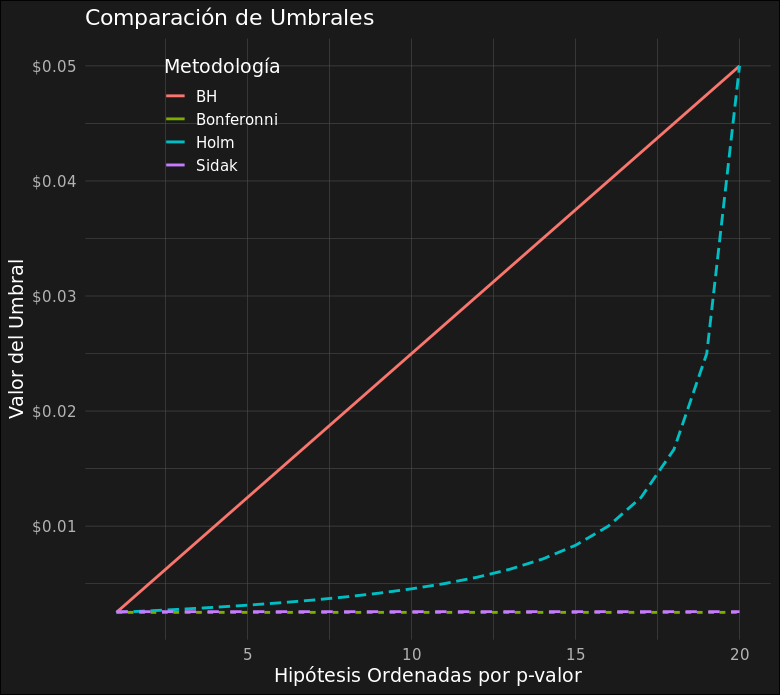
\includegraphics[scale=.5]{comparacion_de_metodos.png}
\caption{Comparación del valor del Umbral de rechazo}
\end{figure}

\subsection{Aplicación del FDR en la ciencia de datos}
\subsubsection{Análisis de ejemplo: Enfermedades relacionadas con la edad influyen en la morfología cerebral}

En este ejemplo, se realizó un análisis de las masas en imágenes de resonancia magnética (RM) extraídas de la iniciativa de datos abiertos de la serie de acceso abierto de estudios de imágenes (OASIS) \cite{cerebro}. Estos datos contienen imágenes ponderadas en T1 de 416 participantes con y sin demencia de entre 18 y 96 años, lo que permite investigar cómo la edad y las enfermedades relacionadas \textbf{con la edad influyen en la morfología cerebral}.\\

Para descargar el conjunto de datos de OASIS, visite $http://www.oasis-brains.org/\#data$ y elija el lanzamiento OASIS-1, que contiene imágenes de resonancia magnética (MR) de 416 participantes de entre 18 y 96 años. El archivo de información del participante incluye variables demográficas básicas (edad, género, mano de obra, nivel educativo, estatus socioeconómico), variables clínicas y estimaciones de volumen cerebral. 

El objetivo del estudio fue determinar que partes del cerebro están relacionadas de su edad. Para probar este hecho se considero calcular los coeficientes de correlación Spearman  entre el grosor cortical y la edad en cada vóxel cortical, y se consideraron 163810 pruebas de la siguiente forma
\begin{align*}
H_{0i}: \rho_s =0 \ \ \ vs \ \ \ H_{0i}:\rho_s\neq 0, \ \ \forall i=1,\cdots, 163810.
\end{align*}
donde $\rho_s=1-\frac{6\sum d_i^2}{n(n^2-1)}$ y $d_i=rg(X_i)-rg(Y_i)$ es la diferencia de los rangos de cada observación. Se puede probar que si $n$ es grande entonces (basado en un argumento de permutación) 
$$\rho_s\sqrt{\frac{n-2}{1-\rho_s^2}} \sim t_{n-2}$$.
Por lo que es sencillo probar significancia con lo anterior. Por lo tanto, considerando lo anterior procedió a calcular los p$-$values de cada juego de hipótesis. Y posterior se le aplicaron las correcciones de Sidák para controlar el family$-$wise error rate (FWER), y el procedimiento BH para controlar la FDR. 
\begin{figure}[H]
\centering \label{cerebro}
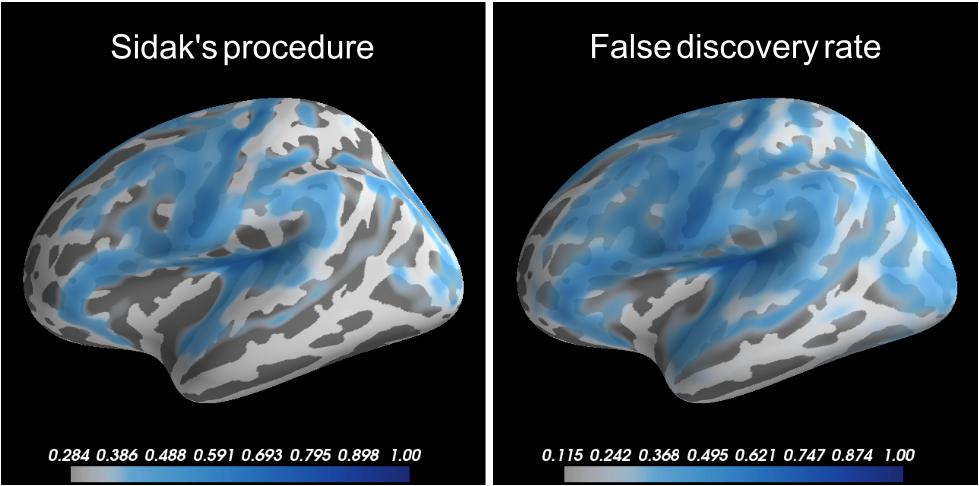
\includegraphics[scale=.5]{neurociencia_FDR_FWER.png}
\caption{Diferencias cuando se controla el FWER y el FDR.}
\end{figure}
Un total del $55\%$ de los vóxel mostró un efecto estadísticamente significativo del envejecimiento sobre el grosor cortical cuando los valores p se corrigieron para múltiples pruebas usando la corrección de Sidak. Por el contrario, cuando la corrección se basó en el procedimiento Benjamini-Hochberg FDR, el número de vértices significativos fue del $82\%$, lo que sugiere un efecto más generalizado. El nivel crítico sin corregir se fijó en $\alpha = 0.05$ en ambos análisis.
Los resultados se muestran en la figura (\ref{cerebro}), lo cuál podemos concluir que algunos de los mayores efectos relacionados con la edad se observan en el surco central \cite{git_cerebro_2}.

\subsubsection{Controling the False-Discovery Rate in Astrophysical Data Analysis.} 

'\textit{El propósito de este artículo es presentar el procedimiento FDR a la comunidad astrofísica. Ilustramos el poder de FDR a través de varios ejemplos astronómicos, incluida la detección de características frente a una función unidimensional suave, por ejemplo, ver las \textit{ondulaciones de bariones} en un espectro de potencia de fluctuaciones de materia y detección de píxeles de origen en datos de imágenes. En esta era de grandes conjuntos de datos y mediciones de alta precisión, FDR proporciona los medios para controlar de manera adaptativa una cantidad cientícamente significativa: la fracción de descubrimientos falsos sobre el total de descubrimientos.}' \cite{Miller_2001}.

\section{Conclusiones}
Se presentaron las bases teóricas sobre las pruebas de hipótesis múltiples desde el enfoque clásico controlando la $FWER$ y la revolucionaria idea que propusieron Benjamini y Hochberh [1995] sobre controlar la $FDR$. Se mostrarón ejemplos en dónde la ventaja sobre controlar la $FDR$ contra $FWER$. Y por lo cual en la actualidad los trabajos referentes a las $MPC$ se centran en controlar estas dos tipos de tasas. La teórica presentada en este documento como se mencionó son las bases de $MCP$, en la actualidad ya existen una gran variedad de metodologías para controlar $FDR$ y $FWER$ la mayoría es son modificaciones del método de Bonferroní y $BH$.\\

Se creé por el estudio realizado que este pequeño campo de conocimiento aún esta por desarrollarse al tal punto aplicarse en diversos temas de ciencias de datos, como los presentados.

\section{Anexo: ANOVA $-$ Pruebas de hipótesis para $k$ proporciones}\label{anexo}
Esta prueba tiene como objetivo probar la hipótesis nula de la igualdad de $\boldsymbol{k}$ proporciones. El procedimiento es el mismo que se utiliza para la prueba de 2 proporciones y consiste en:
\begin{enumerate}[I]
	\item Planteamiento de hipótesis
	$$
	\begin{array}{l}
		\mathrm{H}_{0}: \pi_{1}=\pi_{2}=\ldots =\pi_{k} \\
		\mathrm{H}_{1}: \text{las proporciones poblacionales no son todas iguales}
	\end{array}
	$$
	\item Establecer el nivel de significancia $\alpha$
	\item Estadístico de prueba: el estadístico de prueba ji-cuadrada que se utiliza
	para este tipo de prueba de hipótesis, corresponde a la expresión:
	$$
	\chi_{p}^{2}=\sum \frac{(f_o-f_e)^{2}}{f_e}
	$$
	Con $V=(r-1)(k-1)=k-1$ grados de libertad.
	Siendo, $r= \#$ renglones y $K=\#$ de poblaciones. 	Para calcular las frecuencias esperadas $f_{e}$, para cada una de las celdas que conforman la tabla de
	contingencia es
	$$
	f e=\frac{f_{r}^{*} f_{k}}{n}
	$$
	Donde
	$f_{r}:$ frecuencia total de un renglón determinado
	$f_{k}:$ frecuencia total de una columna determinada
	$n: \quad$ número de observaciones
	4. 
	5. 
	\item Regla de decisión:	$\mathrm{RH}_{0}, \text{ si } \chi_{p}^{2}>\chi_{c r}^{2}$.
	\item Conclusión: también puede recurrir a el cálculo del $p$-valor.
\end{enumerate}

\newpage
\begin{table}[ht]
\centering
\begin{tabular}{c}
\textbf{Ejercio de Tarea. Comparación de Hipotesis Multiples.}\\
\textbf{Inferencia Estadística.} \\
\textbf{Tarea 9}\\
\today
\end{tabular}
\end{table}

Se probaron asociaciones de 25 variables dietéticas  con la densidad mamográfia, el cuál es un factor de riesgo importante para el cáncer de mama en mujeres españolas. Los p-values de las pruebas de hipótesis se encuentran en el archivo \textit{dietary.csv}.\\

\begin{itemize}
    \item Considera los procedimientos descritos en la precentación (Bonferroní, Sidák, Holm-Bonferroni y BH) para controlar las diferentes tasas de error (FWER y FDR).
    
    \item ¿Cuáles es la desición de rechazo para cada metodología? Gráfica los umbrales de rechazo para cada una de las metodología (en una sola gráfica), junto con los p$-$values reales.
    
    \item ¿Qué puedes concluir del experimento sobre las dietas y la densidad mamográfia? 
\end{itemize}

\newpage


\printbibliography


\end{document}